
% ============================================================================================================

% JOURNAL MODE
% ------------

\documentclass[extra]{gji}
\setlength{\paperwidth}{210mm}
\setlength{\paperheight}{297mm}% fixed.
\usepackage[pass]{geometry}\usepackage{timet}

% ============================================================================================================

% MANUSCRIPT MODE
% ---------------

% \documentclass[extra,mreferee]{gji}

% ============================================================================================================

% \addtolength{\paperheight}{1in}

\usepackage{fancyhdr}
\usepackage{comment}
\usepackage{color}
\usepackage{graphicx}
\usepackage{amsmath}
\usepackage{mathtools}
\usepackage{environ}
\usepackage{datatool}
\usepackage{textcomp}


% \widowpenalty=1000
% \clubpenalty=1000


\title[% 
A Comparative Study between CVM-SI.26 and CVMS-4
% 
]{% 
A Comparative Study between Two Versions of Southern California Seismic Velocity Models: CVMS-4 and CVM-SI.26, through Simulation and Validation of Multiple Events
% 

}
\author[R.~Taborda {\rm et al.}]{% 
Ricardo Taborda,$^{1,2}$\thanks{Corresponding author: ricardo.taborda@memphis.edu}
Shima Azizzadeh-Roodpish,$^{1,2}$\vspace{0.5ex} \\ \normalfont{\LARGE and Naeem Khoshnevis,$^{2}$} \vspace{1ex} \\
% 
$^1$ Department of Civil Engineering, University of Memphis, Memphis, TN \emph{38152}, USA\\
$^2$ Center for Earthquake Research and Information, University of Memphis, Memphis, TN \emph{38152}, USA
% 
}
% \date{Received 2015 August 1; in original form 2015 July 1}
\date{To be submitted by June, 2016}
\pagerange{\pageref{firstpage}--\pageref{lastpage}}
\volume{000}
\pubyear{0000}

%\def\LaTeX{L\kern-.36em\raise.3ex\hbox{{\small A}}\kern-.15em
%    T\kern-.1667em\lower.7ex\hbox{E}\kern-.125emX}
%\def\LATeX{L\kern-.36em\raise.3ex\hbox{{\Large A}}\kern-.15em
%    T\kern-.1667em\lower.7ex\hbox{E}\kern-.125emX}
% Authors with AMS fonts and mssymb.tex can comment out the following
% line to get the correct symbol for Geophysical Journal International.

\let\leqslant=\leq

\newtheorem{theorem}{Theorem}[section]


\newcommand{\vsmin}{$V_{S_{\min}}$}
\newcommand{\vsmineq}[1]{$V_{S_{\min}}=#1$~m/s}
\newcommand{\vsthirty}{$V_{S30}$}
\newcommand{\vs}{$V_{S}$}
\newcommand{\vseq}[1]{$V_{S}=#1$~m/s}

\newcommand{\vp}{$V_{P}$}
\newcommand{\vpeq}[1]{$V_{P}=#1$~m/s}

\newcommand{\qp}{$Q_{P}$}
\newcommand{\qs}{$Q_{S}$}

\newcommand{\fleq}[1]{$f\leq#1$~Hz}
\newcommand{\fmax}{$f_{_{\max}}$}
\newcommand{\fmaxeq}[1]{$f_{_{\max}}=#1$~Hz}

\newcommand{\eqmag}[1]{$M_{#1}$}

\newcommand{\adomain}[3]{#1~#3 $\times$ #2~#3}
\newcommand{\vdomain}[4]{#1~#4 $\times$ #2~#4 $\times$ #3~#4}


\begin{document}

\label{firstpage}

\maketitle


\section{Introduction}

Developing community velocity models (CVMs) that can be broadly applied and continuously updated by a community of users has became of interest in simulation-based analysis. CVM-S and CVM-H models, released by Southern California Earthquake Center (SCEC), are good examples of community models, evolved over time. CVM-S, also known as CVM-S4, was originally developed by \citet{Magistrale_1996_BSSA} and later updated by \citet{Magistrale_2000_BSSA} and \citet{Kohler_2003_BSSA}. Recently, a new version of CVM-S, called CVM-S4.26 was built, based on the original model and the results of a sequence of 3D full-waveform tomographic inversions done by \citet{Chen_2007_BSSA} and \citet{Lee_2014_JGR}. CVM-S is known as an acceptable representations of the crustal structure in southern California at low frequencies ($f \leq 0.2$~Hz). According to \citet{Taborda_2016} CVM-S is getting better results than the alternative model CVM-H for the region understudy, even upto 1 Hz, which is in good agreement with previous works done in the area for particular cases (e.g. \citet{Taborda_2014_BSSA} and \citet{Lee_2014_SRL}). There are currently three alternative CVM-SI.26 models (2.2.1, 2.2.2 \& 2.2.3) available which vary depending on how the perturbations were applied to the original model. There have been some researches with the aim of evaluation of different velocity models for southern California region in lower frequencies or for limited number of events. Such differences, however, have never been studied extensively for multiple events and/or at frequencies beyond the upper limits set by the underlying inversions used to construct the models.\par
Here, we design a systematic procedure, through quantitative comparisons among synthetics results of four versions of CVM-S and recorded data of thirty moderate-magnitude events, to evaluate the overall improvement of accuracy in predicting ground motion within simulation domain. The simulations are performed at 1 Hz frequency and minimum shear wave velocity of 200 m/s using Hercules, a finite element application for solving forward wave propagation problems due to kinematic faulting \citep{Tu_2006_Proc, Taborda_2010_Tech}. Comparisions are ranked quantitatively by means of a goodness-of-fit (GOF) criteria at 0.5 Hz, obtained from a modified version of the criteria introduced by \citet{Anderson_2004_Proc}. In the light of the comparision of the regional distribution of the GOF results for all events and all models, We conclude that CVM-SI26.223 consistently yields better results which confirms the improvements in this latest versions.



\section{Study domain and earthquake data}

Considered events for this study, containing thirty moderate-magnitude earthquakes ($3.5 > M_w > 5.5$) occurred between 1998 and 2014, are spread throughout a simulation domain with a volume projection of \vdomain{180}{135}{62}{km}, which covers the entire Los Angeles metropolitan area and most of the significant geologic structures around. (Fig.~\ref{fig:region}) shows the simlation domain in which we labled the events with sequential letter code from A to Z and AA to AD and Table \ref{tab:events} provides detailed information for those selected events.The unprocessed recorded data from Southern California Earthquake Data Center (SCEDC) and Center for Engineering Strong Motion Data (CESMD) are downloaded for each of the earthquakes to take advantage of the numerous time series available from different data centers. We obtained records for moree than 800 stations, Some of which were in common between different networks and some were not usable. Records from SDEDC and CESMD were processed and selected for each event. we performed gain and baseline corrections, and applied a \textcolor{red}{high-pass filter at 0.05 Hz} before integrating to obtain velocities and displacements. The final number of chosen records for validation for any of the selected earthquake can be found in Table \ref{tab:events}. For almost all of the events there is enough available stations to make the results of validation acceptable. 

\begin{figure*}
    \centering
    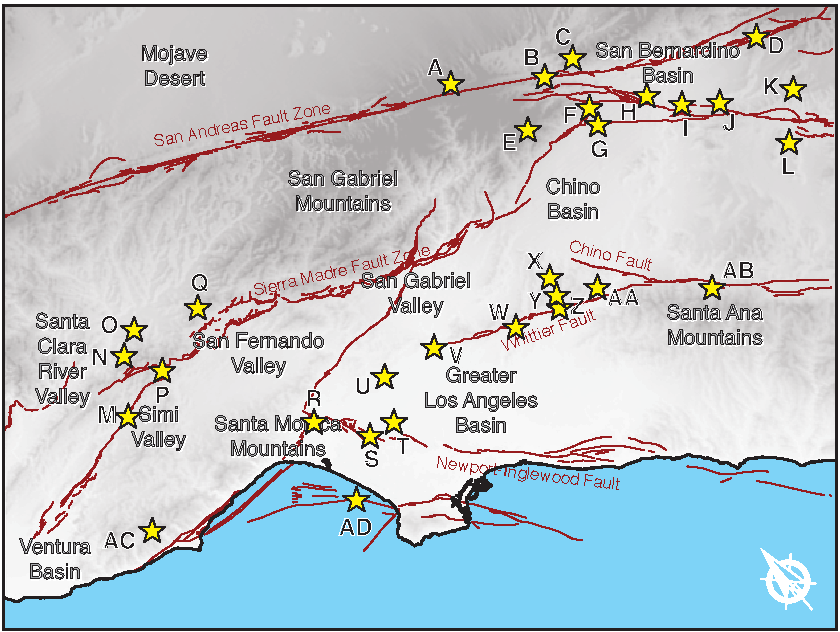
\includegraphics
    	[width=\textwidth]
    	{figures/pdf/figure-01}
    \caption{Region of interest and simulation domain. (a) 3D view of the simulation domain. (b) Geographical location and surface projection of the simulation domain, along with the names of the main cities surrounding the Los Angeles metropolitan are. (c) Major geologic structures including basins, valleys and mountains, along with the main quaternary faults in the region. The color background represents the surface \vsthirty{} values included in the CVM-H+GTL model, with a topography shading effect. The segments $\overline{\mathrm{AB}}$ and $\overline{\mathrm{BC}}$ are used as reference for Fig.~\ref{fig:vslices}.}
    \label{fig:region}
\end{figure*}


\begin{table}
	\centering\small

	\caption{Information for 30 events including their ID \citet{SCEC}, magnitude and final number of stations.}
	\begin{tabular}{|c c c c || c c c c}
	
	\hline

	  	Code								& 
	  	Event ID							& 
	  	\eqmag{w}							&
	  	Num.								&
	  	Code								& 
	  	Event ID							& 
	  	\eqmag{w}							&
	  	Num.								\\
	\hline																																
		A			&	 9064568	&	4.40	&	17&  P&	14312160	&	4.66	&	109	\\ % A 

		B				&	10972299	&	3.79	&	52&	Q&	15237281	&	3.86	&	120\\ % R
		C				&	14494128	&	3.72	&	77&	R&	 9703873	&	4.24	&	130\\ % Z
		D					&	14155260	&	4.88	& 172&	S&	10410337	&	4.70	&	213\\ % V
																					
		E		&	10216101	&	3.60	&	55&	T&	 9716853	&	3.98	&	55\\ % J
																					
		F				&	13692644	&	3.74	&	55&	U&	 9093975	&	3.77	&	25\\ % S
		G				&	14116972	&	4.42	&	83&	V&	14601172	&	4.44	&	180\\ % U
		H			&	10370141	&	4.45	&	159 &	W&	15481673	&	5.10	&	311\\ % L
		I			&	 9140050	&	4.37	&	38&	X&	14383980	&	5.39	&	335\\ % D
		J					&	10541957	& 4.10&	97&	Y&	 9818433	&	4.75	&	67\\ % Q
		K				&	10530013	&	4.28	& 76	& Z&	10399889	&	3.98	&	91\\ % P
		L				&	14239184	&	3.90	&	66&	AA&	 9644101	&	3.64	&	53\\ % W
																					
		M				&	14000376	&	3.59	&	54&	AB&	10275733	&	4.73	&	116\\ % T
		N			&	 9753489	&	3.90	&	52&	AC&	10403777	&	4.42	&	94\\ % H
		O			&	 9096972	&	3.98	&	26&	AD&	14738436	&	3.69	&	93\\ % C
		\hline
																				
	\end{tabular}
	\label{tab:events}
\end{table}






\section{Velocity models and simulation approach}


\input{validation-method}


\section{Ground Motion Simulation Results}

Before we address the evaluation of the models, we present results from the simulations and offer a general perspective on the ground motion characteristics obtained for the events considered. Fig.~\ref{fig:all.pgvs} shows the peak horizontal magnitude of velocity on the free surface for all events, and for the particular case of simulations done using the model CVM-S4.26. This figure illustrates how the basins in the region respond to earthquakes originated at various locations within the simulation domain. Although interpretations in this regard are biased by the choice of the color scale, it is fair to say that earthquakes of magnitude less than 3.9 remain local, showing only a marginal ground response in areas outside their immediate epicentral surrounding (e.g.~events L, M, U). Events of magnitude greater than 4.3, on the other hand, show stronger response all throughout the domain, and exhibit more clearly the effects of the basins (e.g.~events D, P, Y). Events with magnitudes between 3.9 and 4.3 are in a transition zone. In such cases the shallower events register stronger ground motions (e.g.~events Q and Z). 

All events considered, the largest ground motions are obtained for the 2014 \eqmag{w} 5.10 La Habra and 2008 \eqmag{w} 5.39 Chino Hills earthquakes (events W and X, respectively), and the areas with most significant shaking are the greater Los Angeles basin, the San Bernardino basin and the region between Simi valley and the Ventura basin. While Fig.~\ref{fig:all.pgvs} only includes results obtained using CVM-S4.26, these observations are consistent across velocity models. We, however, now focus our attention to the discrepancies observed when using different velocity models. 

\begin{figure*}
    \centering
    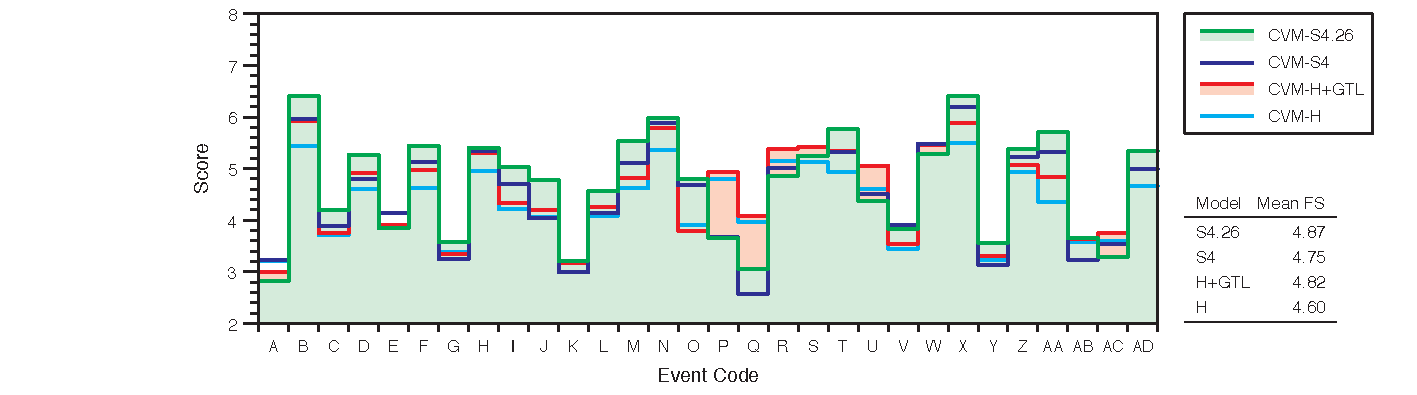
\includegraphics
        [width=\textwidth]
        {figures/pdf/figure-06}
    \caption{Free surface peak horizontal magnitude velocity from simulations for all the events using the velocity model CVM-S4.26. The letter code used to identify each earthquake is shown at the top-left corner along with the event's magnitude, \eqmag{w} (see Table \ref{tab:events}). In each case, the star indicates the epicenter of the event (see also Fig.~\ref{fig:epicenters}). Although smaller and larger values than those shown in the color scale were obtained from the simulations, these were truncated for visual convenience.}
    \label{fig:all.pgvs}
\end{figure*}

\begin{figure*}
    \centering
    \includegraphics
        [width=\textwidth]
        {figures/pdf/figure-07}
    \caption{Free surface peak horizontal magnitude velocity for three representative events (from top to bottom: G, W, and P) using all four velocity models (from left to right: CVM-S4, CVM-S4.26, CVM-H and CVM-H+GTL). The stars indicate the epicenter locations (see Table \ref{tab:events} and Fig.~\ref{fig:epicenters} for reference). In each case, smaller and larger values than those shown in the contour maps were obtained, but truncated for visual convenience.}
    \label{fig:selected.pgvs}
\end{figure*}

Fig.~\ref{fig:selected.pgvs} shows the peak horizontal magnitude of velocity on the free surface for all velocity models, for the particular cases of the 2005 \eqmag{w} 4.42 Fontana, 2007 \eqmag{w} 4.66 Chatsworth, and 2014 \eqmag{w} 5.10 La Habra earthquakes (events G, P, and W, respectively). We select these three events for their location and magnitudes above 4, with well spread response over the simulation domain. The Fontana (G) earthquake epicenter was located in the northern section of the San Jacinto fault zone, not far from the junction with the San Andreas fault zone and the Cucamonga fault (see Fig.~\ref{fig:epicenters}). This earthquake shows clear influence in the area of the San Bernardino basin for all four models, although with some differences. In the case of CVM-S4, for instance, a significant level of the response is channeled into the Chino and the greater Los Angeles basins, as well as far into the Simi and the Santa Clara river valleys. A similar response is seen in the case of CVM-S4.26, but to a lesser extend, with only marginal response in the Santa Monica area. CVM-S4.26 also exhibits lower values southwest and northwest fromt he epicenter than CVM-S4. In the cases of CVM-H and CVM-H+GTL, the ground motion is more localized around the epicentral area. Both models, however, seem to channel more energy along the north flank of the San Andreas Fault and to the south east and south west, in particular along the west edge of the Santa mountains, where both CVM-H and CVM-H+GTL have deeper structures than CVM-S4 or CVM-S4.26 (see Fig.~\ref{fig:hslices} for reference).

In the case of the Chatsworth earthquake, the strongest response concentrates in the Simi and San Fernando valleys, along the Santa Clara river valley and into the Ventura basin. For the simulations done with CVM-S4 and CVM-S4.26, however, a greater amount of energy is channeled west into the Ventura basin and southeast towards the greater Los Angeles area. Both CVM-S4 and CVM-H show some level of basin effects in San Bernardino, an area where CVM-H+GTL shows the least level of amplification of all the models, due to the changes introduced by the GTL model as highlighted in Fig.~\ref{fig:vslices}. Both CVM-H and CVM-H+GTL show a stronger contrast between the Simi and San Fernando valleys and the Los Angeles basin, marked by the influence of the Santa Monica mountains, which seem to be more sharply defined in these two models than in CVM-S4 and CVM-S4.26 (see Fig.~\ref{fig:hslices}).

Last, in the case of the La Habra earthquake, the ground motions are mostly concentrated in the greater Los Angeles basin, though with some significant differences amongst the models. We first note again the fact that the model CVM-H+GTL introduces strong changes in the response of the San Bernardino basin with respect to CVM-H. As in other cases, CVM-H and CVM-H+GTL yield larger ground motions in the area of Irving (see Fig.~\ref{fig:region}) southeast from the epicenter. CVM-S4 and CVM-S4.26, on the other hand, exhibit larger ground motions within the Los Angeles basin itself and in the Chino basin. In turn, CVM-S4.26 yields larger shaking near the San Gabriel valley and mountains, and beyond in the Mojave desert. CVM-S4.26 also exhibits stronger response in the area of the Santa Ana mountains, as a result of the contrast in the model in this area with respect to CVM-S4. Of all four models, CVM-S4 has stronger response in the Ventura basin and CVM-H along the Santa Clara river valley---which likely reflects a better coupling between the crustal structure and faults representation in the model, considering the weak zone along the Santa Clara river due to the presence of the Oak Ridge fault beneath it.

Although not in equal measure for all events, the differences just highlighted were common among the models in the simulation results of other earthquakes. We further analyze the implications of these model discrepancies and their consequence in simulation results through the validation of synthetics against data in the following sections.





\section{Evaluation Method}

The validation process consists of comparisons between processed data and synthetics, at locations where records were available for the simulated events. This was carried out using the goodness-of-fit (GOF) method proposed by \citet{Anderson_2004_Proc}, with minor modifications introduced by \citet{Taborda_2013_BSSA}. The method compares synthetics against data using eleven individual parameters, namely: Arias intensity integral (C1), energy integral (C2), Arias intensity value (C3), total energy (C4), peak acceleration (C5), peak velocity (C6), peak displacement (C7), response spectrum (C8), Fourier amplitude spectrum (C9), cross correlation (C10), and strong-phase duration (C11). Each parameter is mapped onto a numerical scale ranging from 0 to 10, where a score of 10 corresponds to a perfect match between two signals. The values obtained for a given pair of signals for each of the eleven scores are combined using the expression: 
%
\begin{equation}
	\mathrm{S} = \frac{1}{9} \left( 
		\frac{\mathrm{C}1+\mathrm{C}2}{2} +
		\frac{\mathrm{C}3+\mathrm{C}4}{2} +
		\sum_{i=5}^{11} \mathrm{C}i
	\right)
	\hspace{0.25em}.
	\label{eq:s}
\end{equation}

Following the guidelines suggested by \citet{Anderson_2004_Proc}, this scoring procedure is applied to each pair of data and synthetics using compatible ``broadband'' sets, and a series of band-pass filtered versions of the signals or sub-bands, SB$_1$, SB$_2$, and SB$_3$. The results of S from equation (\ref{eq:s}) for the broadband (BB) and each of the sub-bands (SB$_i$) are then combined to obtain a final score (FS), define as:
%
\begin{equation}
	\mathrm{FS} = \frac{1}{4} \left( \mathrm{BB} + \sum^3_{i=1} \mathrm{SB}_i \right)
	\hspace{0.25em}.
	\label{eq:fs}
\end{equation}

We used signals band-pass filtered between 0.1 and 1.0 Hz for BB, and between 0.1 and 0.25~Hz, 0.25 and 0.5~Hz, and 0.5 and 1~Hz for SB$_1$, SB$_2$, and SB$_3$, respectively. The upper frequency limit of 1~Hz was based on the maximum frequency of the simulations. The lower limit of 0.1~Hz, on the other hand, was determined by the need for minimizing instrumental and numerical processing issues at the low frequencies (0--0.1~Hz), which can be introduced when processing strong motion and broadband records to obtain velocities and displacements. This also helps eliminate permanent displacements in the synthetics extracted at locations near the epicenter, especially for shallower earthquakes. 

Before running the comparison process, signals are also (sub)-sampled to have the same time-step size, $\Delta t$. We chose a common $\Delta t$ equal 0.1 s, and used a decimation corner (low-pass) frequency of 2~Hz for the records. This corresponds to a Nyquist frequency of 5~Hz, or five times the simulation maximum frequency. In addition, both data and synthetics were synchronized using the earthquake times (shown in Table \ref{tab:events}) as reference. Synthetics were synchronized assuming that the earthquake time corresponds to the instant at which the source slip-time function is at half the total rise time. Data were synchronized using the time-stamp on the record. We cut or zero-padded the records at the beginning depending on whether the station channel started recording before or after the earthquake time. When zero-padding, a tapper filter in time was applied at the beginning of the record. Once the signals have been synchronized in terms of start-time, they are also matched to have the same length, using the shortest of the two to determine the length used for comparisons. Applying these filters equally to data and synthetics, using a common $\Delta t$, and synchronizing the start- and end-time of each pair of signals provides a maximum level of consistency in both the frequency and time domains, which minimizes the numerical discrepancies that could arise from the comparisons performed using the different metrics C1 through C11.

Additional details about the original parameters proposed by \citet{Anderson_2004_Proc} and the modifications introduced to the scoring criterion are given in \citet{Taborda_2013_BSSA}. \citet{Taborda_2013_BSSA, Taborda_2014_BSSA} also include brief discussions regarding the choice of the method proposed by \citet{Anderson_2004_Proc}, in light of other available procedures such as those introduced by \citet{Kristekova_2006_BSSA}, \citet{Kristekova_2009_GJI} or \citet{Olsen_2010_SRL}. In summary, previous experience in verification and validation efforts tells us that the method of \citet{Anderson_2004_Proc} works better for validation, as opposed to verification, mainly because it is not restricted to matching waveforms, but is rather oriented at conveying information of physical meaning to both seismologists and engineers. We also prefer \citet{Anderson_2004_Proc} because it provides additional consistency with respect to previous work done by \citet{Taborda_2013_BSSA, Taborda_2014_BSSA}.
 


\section{Data Processing}

The unprocessed recorded data of different networks from SCEC and Strong motion are downloaded for each of the events to take advantage of the numerous time series available from different data centers.

Some of the stations were in common between different networks and some of them were not usable and they needed to be removed. 
The total number of stations available from different networks and the final number of chosen records  for validation for any of the selected earthquake is presented in table 2.  
As it shows, only two events, Chino Hills and Lahabra, have a large number of recorded data. Still, for almost all of the events there is enough  available stations to make the results of validation acceptable. 




\section{Analysis of Results}

The observations are helpful in identifying region where the velocity model may need to be revised. 



\section{Conclusions}

The main research goal of the proposed activities is to evaluate the different available velocity models.
Our results for the goodness-of fit measure of the synthetics indicate that, CVMS4.26 shows an overall improvement for all the events.   


%
\begin{acknowledgments}
% 
This work was supported by the United States Geological Survey (USGS) through the award ``Evaluation of the southern California seismic velocity models through ground motion simulation and validation of past earthquakes'' (G14AP00034); and by the Southern California Earthquake Center (SCEC) through the award ``Evaluation of CVM-SI.26 perturbations integration involving undergraduate computer science and graduate earth sciences and engineering students'' (14032). Additional support was provided through the U.S.~National Science Foundation (NSF) award ``SI2-SSI: A Sustainable Community Software Framework for Petascale Earthquake Modeling'' (ACI-1148493). This research is also part of the Blue Waters sustained-petascale computing project, which is supported by NSF (awards OCI-0725070 and ACI-1238993) and the state of Illinois. Blue Waters is a joint effort of the University of Illinois at Urbana-Champaign and its National Center for Supercomputing Applications (NCSA). Computational support was possible through PRAC allocations supported by NSF awards ``Petascale Research in Earthquake System Science on Blue Waters (PressOnBlueWaters)'' (ACI-0832698); and ``Extending the spatiotemporal scales of physics-based seismic hazard analysis'' (ACI-1440085). SCEC is funded by NSF Cooperative Agreement EAR-1033462 and USGS Cooperative Agreement G12AC20038. The SCEC contribution number for this paper is \textcolor{red}{PEDNING}.
% 
\end{acknowledgments}






\bibliographystyle{gji}
\bibliography{references}
% \bsp 

\label{lastpage}

\end{document}
